%Chapter 1
\chapter{Introduction}\label{sec:introduction}

\section{Background: The Startup Dilemma}\label{sec:background}
The modern software startup ecosystem embodies a fundamental tension between two competing engineering philosophies. On one side stands Facebook's notorious "move fast and break things" ethos, championing rapid iteration and accepting imperfect code as a necessary cost of market velocity. On the other, traditional software engineering wisdom advocates for the "slow down and build it right" principle, emphasizing careful design and sustainable development practices.

This philosophical divide becomes particularly acute when examining venture execution, defined here as a startup's ability to rapidly iterate and deliver software features at a pace that demonstrates momentum to investors \citep{gompers2001venture, lee2024startups}, operationalized through development velocity and market validation via successful funding rounds. Development velocity represents the technical dimension of how rapidly a team can iterate and deploy features, while technical debt accumulation reflects the engineering trade-offs made in pursuit of such speed \citep{cunningham1992wycash, besker2018embracing}.

Technical debt, a metaphor introduced by Ward Cunningham to describe the implied cost of choosing an expedient solution instead of a better approach \citep{cunningham1992wycash}, manifests in shortcuts in code architecture, deferred refactoring, inadequate documentation, and accumulated complexity. While conventional software engineering literature universally characterizes technical debt as detrimental to long-term productivity, this perspective may not adequately account for the unique strategic context faced by resource-constrained startups.

Venture-backed software companies operate under extraordinary pressure for rapid growth and milestone achievement, with funding rounds serving as critical validation points for survival and continued capital access \citep{sahlman1990structure}. Staged financing allows investors to mitigate risk by evaluating startups at discrete milestones, with each successful round signaling market traction and reducing information asymmetry \citep{levesque2000effects, gompers2001venture}. The post-2008 macroeconomic environment, characterized by the Federal Reserve's \ac{ZIRP}, fundamentally altered this dynamic. During the \ac{ZIRP} era (c. 2009-2022), near-zero interest rates flooded the startup ecosystem with abundant capital \citep{ning2015driving}, creating a "growth-at-all-costs" environment where rapid execution often superseded operational efficiency \citep{kuratko2020blitzscaling}. This context was intensified by the compression of competitive windows: the average time between product introduction and competitive entry contracted from 33 years in the early 20th century to just 3.4 years for recent innovations \citep{agarwal2001first}, making first-mover advantages increasingly valuable \citep{lieberman1998first}. Under these conditions, aggressive technical debt accumulation became a potentially rational strategic choice—a form of temporal arbitrage where organizations trade future development efficiency for immediate execution capability when current capacity is demonstrably more valuable than equivalent future capacity \citep{besker2018embracing}.

\section{Problem Statement}\label{sec:problem}

Despite the prevalence of technical debt discussions in both academic literature and industry discourse, there exists a significant gap in empirical understanding of its actual impact on venture execution and funding success, particularly within the unique macroeconomic context of the \ac{ZIRP} era. Technical debt has been extensively studied within software engineering \citep{li2015systematic}, and startup development practices have been examined in entrepreneurship literature \citep{klotins2019software, nguyen2021entrepreneurial, besker2018embracing}. However, these research streams have largely evolved in parallel. Venture capital evaluation literature analyzes funding determinants \citep{gompers2001venture, lee2024startups} but treats technical execution as a black box. As illustrated in Figure \ref{fig:research_gap}, this thesis addresses the intersection of these domains, examining how technical debt accumulation and development velocity associate with funding success in the capital-abundant \ac{ZIRP} era.

\begin{figure}[htbp]
\centering
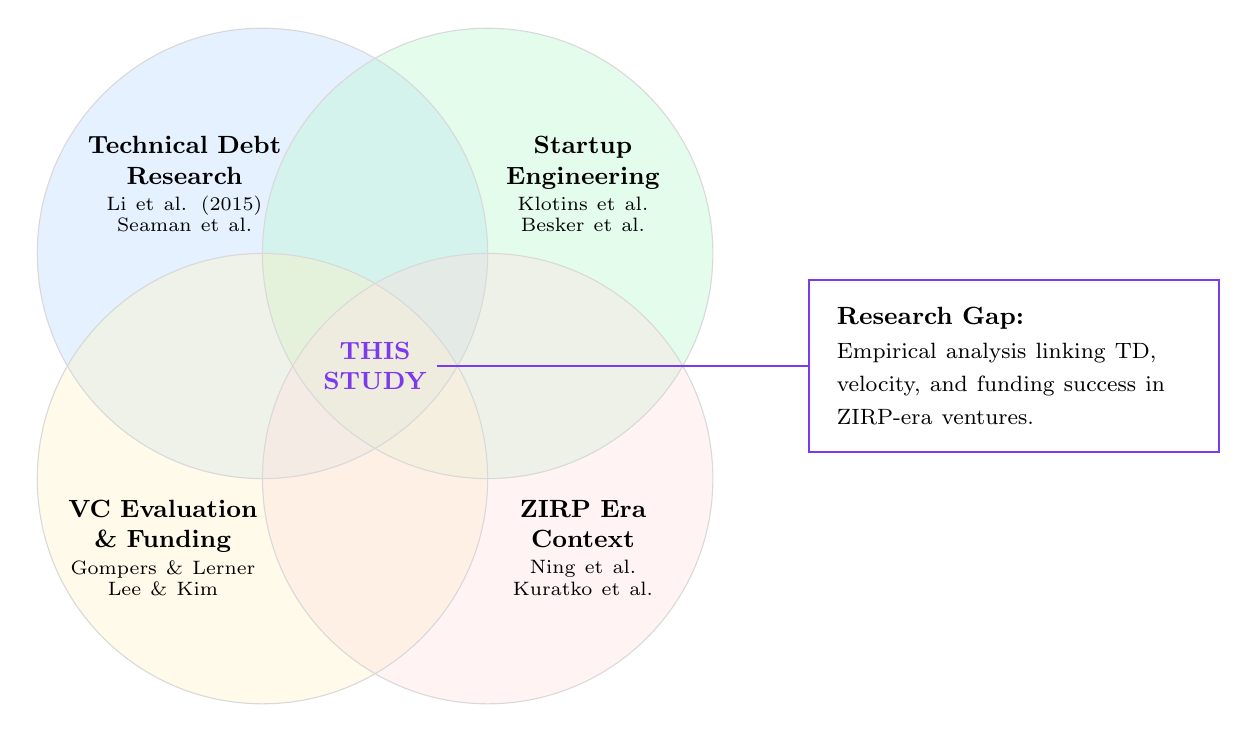
\begin{tikzpicture}[scale=1.1]
    % Define professional pastel colors
    \definecolor{techdebt}{RGB}{191, 219, 254}    % Soft Blue
    \definecolor{startup}{RGB}{187, 247, 208}     % Soft Green
    \definecolor{vcfunding}{RGB}{254, 243, 199}   % Soft Amber
    \definecolor{zirpera}{RGB}{254, 226, 226}     % Soft Red
    \definecolor{gapcolor}{RGB}{124, 58, 237}     % Vibrant Purple
    
    % Draw four overlapping circles - Radius increased to 2.6cm for better text fit
    \begin{scope}[fill opacity=0.4]
        \fill[techdebt] (-1.3,1.3) circle (2.6cm);
        \fill[startup] (1.3,1.3) circle (2.6cm);
        \fill[vcfunding] (-1.3,-1.3) circle (2.6cm);
        \fill[zirpera] (1.3,-1.3) circle (2.6cm);
    \end{scope}

    % Thin borders for crisp definition
    \draw[gray!30, thin] (-1.3,1.3) circle (2.6cm);
    \draw[gray!30, thin] (1.3,1.3) circle (2.6cm);
    \draw[gray!30, thin] (-1.3,-1.3) circle (2.6cm);
    \draw[gray!30, thin] (1.3,-1.3) circle (2.6cm);
    
    % Internal labels - Moved inward to (2.1, 2.1) for perfectly even padding
    % Citation spacing tightened aggressively with [-1.4ex]
    \node[text width=3.2cm, align=center] at (-2.2,2.1) {
        \small\textbf{Technical Debt}\\
        \small\textbf{Research}\\[0.05cm]
        \scriptsize Li et al. (2015)\\[-1.4ex]
        \scriptsize Seaman et al.
    };
    
    \node[text width=3.2cm, align=center] at (2.4,2.1) {
        \small\textbf{Startup}\\
        \small\textbf{Engineering}\\[0.05cm]
        \scriptsize Klotins et al.\\[-1.4ex]
        \scriptsize Besker et al.
    };
    
    \node[text width=3.2cm, align=center] at (-2.45,-2.1) {
        \small\textbf{VC Evaluation}\\
        \small\textbf{\& Funding}\\[0.05cm]
        \scriptsize Gompers \& Lerner\\[-1.4ex]
        \scriptsize Lee \& Kim
    };
    
    \node[text width=3.2cm, align=center] at (2.4,-2.1) {
        \small\textbf{ZIRP Era}\\
        \small\textbf{Context}\\[0.05cm]
        \scriptsize Ning et al.\\[-1.4ex]
        \scriptsize Kuratko et al.
    };
    
    % Central text - Focal point in bold purple, background-free
    \node[align=center, font=\bfseries\small, text=gapcolor] (centertext) at (0,0) {THIS\\STUDY};
    
    % Vertically centered Research Gap box - Sharp formal corners
    \node[anchor=west, text width=4.5cm, draw=gapcolor, thick, fill=white, inner sep=10pt] (gapbox) at (5.0, 0) {
        \textbf{\small Research Gap:}\\
        \footnotesize Empirical analysis linking TD, velocity, and funding success in ZIRP-era ventures.
    };

    % Connection line - Clean, minimalist, no arrowhead
    \draw[thick, gapcolor] (centertext.east) -- (gapbox.west);
    
\end{tikzpicture}
\caption{Research Gap at the Intersection of Technical Debt, Startup Strategy, VC Funding, and ZIRP-Era Context}
\label{fig:research_gap}
\end{figure}

While \citet{besker2018embracing} and \citet{cico2021toward} have explored technical debt in startup contexts through qualitative interviews and case studies, no prior research has systematically quantified these relationships across multiple companies and funding cycles, nor examined how macroeconomic conditions moderate the strategic implications of engineering trade-offs. The existing research predominantly relies on anecdotal evidence or small-N case studies that may not adequately capture the complex trade-offs faced by venture-backed startups operating under capital abundance and time pressure.

This research gap is particularly problematic given the substantial resources allocated to technical debt management in the startup ecosystem and the potential strategic implications for both entrepreneurs and \ac{VC} investors. Without empirical evidence of technical debt's actual impact on business outcomes in the \ac{VC} context, stakeholders lack the quantitative foundation necessary to make informed decisions about resource allocation between code quality maintenance and feature development velocity.

\section{Research Question}\label{sec:research_questions}

This thesis addresses a central strategic question for venture-backed software companies:

\textbf{Research Question}: How do technical debt accumulation and development velocity, individually and in combination, associate with a startup's ability to secure subsequent rounds of funding?

This question encompasses two analytical components that inform the strategic framework. First, examining whether technical debt systematically constrains development velocity tests the conventional assumption that debt creates ``interest payments'' limiting execution speed. Second, analyzing how debt-velocity combinations predict funding success reveals which strategic positions enable venture outcomes during the ZIRP era. The research design treats technical debt and development velocity as organizational choices that may interact to influence investor confidence and capital access.

\section{Contribution of this Thesis}\label{sec:contribution}

This research makes three primary contributions to the fields of software engineering and entrepreneurship:

\textbf{Methodological Innovation}: The creation of a novel, automated analysis pipeline capable of conducting longitudinal analysis of code quality and development velocity in startup environments. This pipeline enables systematic examination of technical debt accumulation patterns across multiple companies and funding periods, providing a scalable approach for future research in this domain.

\textbf{Scientific Reproducibility and Open Data}: This research establishes a replicable foundation for quantitative startup studies by making the underlying dataset and automated analysis pipeline publicly available. By providing a verifiable benchmark through the longitudinal analysis of 70 open-source \ac{VC}-backed companies, the study offers a standardized framework for the research community to validate these findings or adapt the methodology to analyze emerging post-\ac{ZIRP} economic environments.

\textbf{Strategic Framework}: Proposing a strategic framework for understanding technical debt in an entrepreneurial context that acknowledges the legitimacy of debt accumulation as a rational choice under specific macroeconomic and competitive conditions. This framework challenges the universally negative characterization of technical debt in traditional software engineering literature by demonstrating context-dependent outcomes.

The research employs the established Technical Debt Ratio (\acs{TDR}) calculation methodology for measuring code quality, while development velocity is assessed through a composite metric building upon the Cloud Native Computing Foundation's approach to measuring open source project velocity, incorporating code churn, commit frequency, and team engagement patterns.

\vspace{1cm}

\begin{figure}[htbp]
\centering
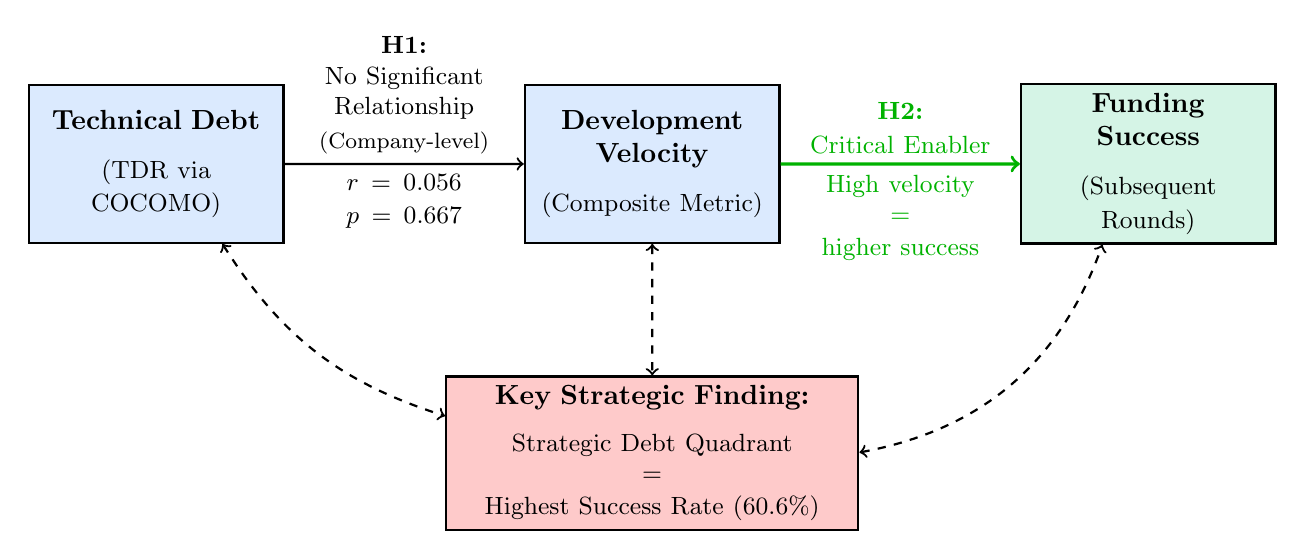
\begin{tikzpicture}[scale=1.05]
    % Define colors from quadrant graphic
    \definecolor{lightblue}{RGB}{219, 234, 254}
    \definecolor{lightgreen}{RGB}{213, 244, 230}
    \definecolor{lightred}{RGB}{254, 202, 202}
    
    % Main variables - repositioned for better spacing
    \node[draw, thick, fill=lightblue, text width=3cm, align=center, minimum height=2cm] (TD) at (0,1) {
        \textbf{Technical Debt}\\[0.2cm]
        \small (TDR via COCOMO)
    };
    
    \node[draw, thick, fill=lightblue, text width=3cm, align=center, minimum height=2cm] (DV) at (6,1) {
        \textbf{Development}\\
        \textbf{Velocity}\\[0.2cm]
        \small (Composite Metric)
    };
    
    \node[draw, thick, fill=lightgreen, text width=3cm, align=center, minimum height=2cm] (FS) at (12,1) {
        \textbf{Funding}\\
        \textbf{Success}\\[0.2cm]
        \small (Subsequent Rounds)
    };
    
    % Main relationship arrows with proper findings - structured labels
    \draw[thick, ->] (TD) -- (DV) 
        node[midway, above, text width=2.5cm, align=center] {
            \small\textbf{H1:}\\
            \small No Significant\\
            \small Relationship \\
            \footnotesize (Company-level)
        }
        node[midway, below, text width=2.5cm, align=center] {
            \small $r = 0.056$\\
            \small $p = 0.667$
        };
    
    \draw[very thick, ->, green!70!black] (DV) -- (FS) 
        node[midway, above, text width=3cm, align=center] {
            \small\textbf{H2:}\\
            \small Critical Enabler
        }
        node[midway, below, text width=3cm, align=center] {
            \small High velocity\\
            \small = \\
            \small higher success
        };
    
    % Strategic insight box - moved lower for better spacing
    \node[draw, thick, fill=lightred, text width=5cm, align=center, minimum height=1.5cm] (KEY) at (6,-2.5) {
        \textbf{Key Strategic Finding:}\\[0.2cm]
        \small Strategic Debt Quadrant\\
        \small = \\
        \small Highest Success Rate (60.6\%)
    };
    
    % Connect key finding to main variables
    \draw[thick, <->, dashed] (TD) to[bend right=20] (KEY);
    \draw[thick, <->, dashed] (DV) to[left=0] (KEY);
    \draw[thick, <->, dashed] (KEY) to[bend right=30] (FS);
    
\end{tikzpicture}
\caption{Conceptual Framework - Development Velocity as Primary Success Driver}
\label{fig:conceptual_framework}
\end{figure}

\section{Thesis Outline}\label{sec:outline}

The remainder of this thesis is structured as follows:

\textbf{Chapter 2: Literature Review} situates this work within existing academic and industry conversations, examining the theoretical foundations of technical debt measurement, development velocity assessment, and venture capital success metrics. This chapter establishes the conceptual framework underlying the empirical analysis and identifies specific gaps that this research addresses.

\textbf{Chapter 3: Methodology} provides a comprehensive account of the research design, data collection procedures, and analytical methods employed. This chapter details the automated analysis pipeline, including sample selection criteria, technical debt measurement using the Qlty platform, development velocity calculation methodology, and statistical analysis approaches.

\textbf{Chapter 4: Results} presents the empirical findings objectively, including the analysis of technical debt and development velocity relationships through both per-period and per-company approaches, performance analysis across strategic quadrants, and funding success patterns observed across the 146 funding periods analyzed.

\textbf{Chapter 5: Discussion} interprets the results within the broader context of software engineering and entrepreneurship literature, with particular attention to the implications of the non-significant correlation between technical debt and velocity, and the finding that high-velocity development emerged as a strong predictor of funding success, with the strategic debt quadrant (high debt + high velocity) achieving the highest success rate at 60.6\%.

\textbf{Chapter 6: Conclusion} summarizes the key findings, acknowledges the limitations of the study, and proposes avenues for future research, including the need to examine whether these relationships hold in post-\ac{ZIRP} economic environments characterized by capital scarcity and altered investor priorities.